% Created 2013-06-26 Wed 11:16
\documentclass[bigger]{beamer}
\usepackage[utf8]{inputenc}
\usepackage{hyperref}
\usepackage{graphicx}
\usepackage{longtable}
\usepackage{float}
\mode<beamer>{\usetheme{Madrid}}
\usepackage{verbatim}
\usepackage{color}
\usepackage{amsmath,amsfonts,amssymb}
\providecommand{\alert}[1]{\textbf{#1}}

\title{Open Software - Restricted Data:  A Suicide/Climate Case Study.}
\author{Ivan Hanigan$^1$, David Fisher$^2$, Steven McEachern$^3$}
\date{June 26, 2013}
\hypersetup{
  pdfkeywords={},
  pdfsubject={},
  pdfcreator={Emacs Org-mode version 7.9.3f}}

\institute[NCEPH]{$^1$National Centre for Epidemiology and Population Health (ANU) \\ $^2$Information Technology Services (ANU) \\ $^3$Australian Data Archives (ANU)}
\begin{document}

\maketitle

% Org-mode is exporting headings to 3 levels.



\section{Aim}
\label{sec-1}
\begin{frame}
\frametitle{Aim}
\label{sec-1-1}

\begin{itemize}
\item Restrictions on data access have increased recently
\item Concerns regarding reproducibility of data analyses
\item Access to data and analytic software addresses the:\\
 \textbf{Replicability Crisis}, (Peng 2011, \emph{Science}, 334;6060)
\item We built a safe Sever/Client IT environment for this
\item We show a Case Study of Suicide and Climate Impacts research
\end{itemize}
\end{frame}
\section{Methods}
\label{sec-2}
\begin{frame}
\frametitle{Methods}
\label{sec-2-1}

\begin{figure}[!h]
\centering
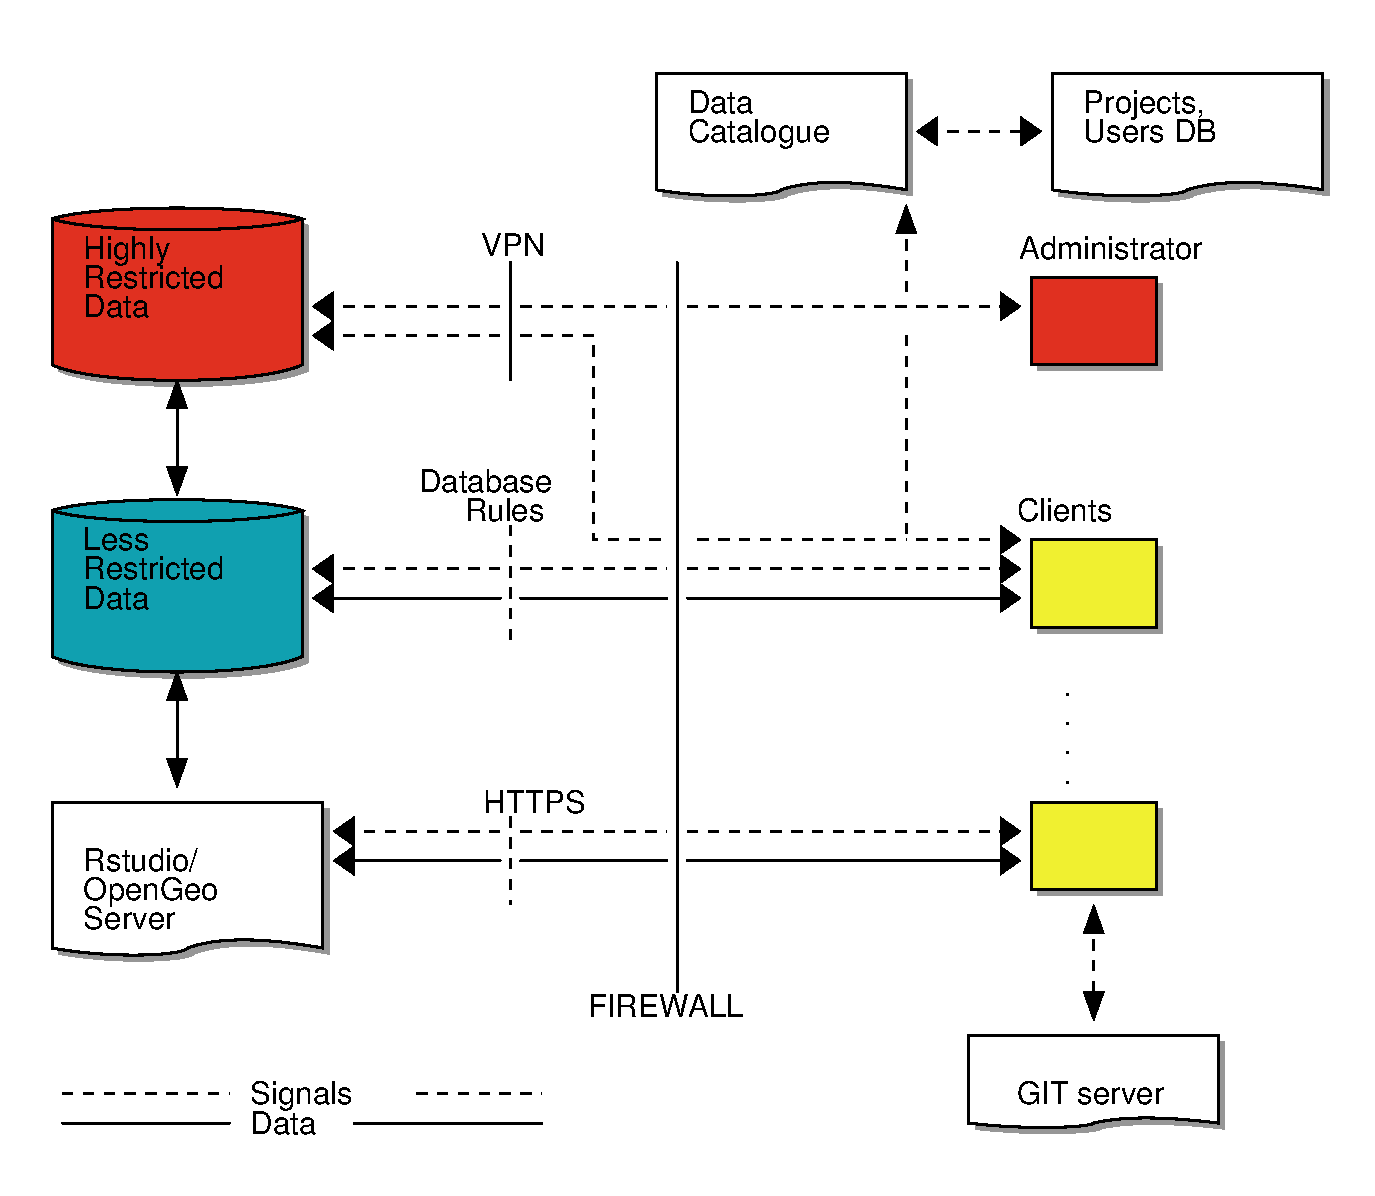
\includegraphics[width=.65\textwidth]{opensoft.pdf}
\caption{1. System Design}
\label{fig:sys}
\end{figure}
\end{frame}
\section{Results}
\label{sec-3}
\begin{frame}
\frametitle{Results (Hanigan et al, 2012, \emph{PNAS}, 109;35)}
\label{sec-3-1}

\begin{footnotesize}
\begin{itemize}
\item {\color{red}Restricted Health and Climate data} and 
\item {\color{blue}Less Restricted Population data} 
\end{itemize}
(Colours refer to data storage and access rules shown in Figure 1).
\begin{eqnarray*}
        log({\color{red} O_{ijk}})  & = & s({\color{red}ExposureVariable})  + {\color{blue} OtherExplanators}  \\
        & &   + AgeGroup_{i} + Sex_{j} \\
        & &   + {\color{blue} SpatialZone_{k}}  \\
        & &  + sin(Time \times 2 \times \pi) + cos(Time \times 2 \times \pi) \\
        & &  + Trend \\
        & &   + offset({\color{blue} log(Pop_{ijk})})\\
\end{eqnarray*}
\end{footnotesize}
\begin{tiny}
\noindent Where:\\
        \indent ${\color{red}O_{ijk}}$ = Outcome (counts) by Age$_{i}$, Sex$_{j}$ and SpatialZone$_{k}$ \\
        \indent {\color{red}ExposureVariable} = Data with {\color{red}Restrictive Intellectual Property~(IP)} \\
        \indent {\color{blue}OtherExplanators} = Other {\color{blue}Less Restricted}  Explanatory variables \\
        \indent s( ) = penalized regression splines \\
        \indent ${\color{blue} SpatialZone_{k}}$  = {\color{blue} Less Restricted} data representing the $SpatialZone_{k}$  \\
        \indent Trend = Longterm smooth trend(s) \\
        \indent ${\color{blue}Pop_{ijk}}$ = interpolated Census populations, by time in each group\\
\end{tiny}
\end{frame}
\begin{frame}
\frametitle{Future (Bambrick et al, 2008, Garnaut Review)}
\label{sec-3-2}

\begin{footnotesize}
$$Y_{ijk}=\sum_{lm}(e^{(\beta_{ijk} \times {\color{red} X_{lm}})} - 1) \times {\color{red}BaselineRate_{jkl}} \times {\color{blue} Population_{jklm}}$$
\noindent Where:\\
$\beta_{ijk}$ = the ExposureVariable coefficient for zone$_i$, age$_j$ and sex$_{k}$ \\
${\color{red}X_{lm}}$ = Projected Future ExposureVariables {\color{red} with Restrictive IP} \\
{\color{red}BaselineRate$_{jkl}$} = {\color{red}avgDeathsPerTime}/{\color{blue}avgPopPerTime} in age$_j$, sex$_k$ and zone$_l$ \\
{\color{blue}Population$_{jklm}$} = projected populations by age$_j$, sex$_k$, zone$_l$ and time$_m$ {\color{blue} (With Less Restrictions)}\\

\end{footnotesize}
\end{frame}
\section{Conclusion}
\label{sec-4}
\begin{frame}
\frametitle{Conclusion}
\label{sec-4-1}

This system:
\begin{itemize}
\item Enables data analysis in a safe environment
\item Allows comparison of multiple climate scenarios and assumptions
\item Demonstrated with a Climate/Health Impact Assessment
\end{itemize}
\begin{itemize}
\begin{large}
\item And this is Reproducible
\end{large}
\end{itemize}
\end{frame}
\section{Acknowledgements}
\label{sec-5}
\begin{frame}
\frametitle{Acknowledgements}
\label{sec-5-1}


\includegraphics[width=4cm]{ANU_LOGO_cmyk_56mm.png}

\includegraphics[width=3cm]{andslogo.pdf}

\includegraphics[width=3cm]{deptlogo.pdf} \\
\begin{footnotesize}
This project is supported by the Australian National Data Service through the National Collaborative Research Infrastructure Strategy Program and the Education Investment Fund (EIF) Super Science Initiative.

More information from:
\begin{itemize}
\item \texttt{ivan.hanigan@gmail.com}
\item \texttt{http://opensoftware-restricteddata.github.io}
\end{itemize}
\end{footnotesize}
\end{frame}
\section{References}
\label{sec-6}
\begin{frame}
\frametitle{References}
\label{sec-6-1}

\begin{footnotesize}
\begin{thebibliography}{1}

\bibitem{Peng2011}
Roger~D Peng.
\newblock {Reproducible research in computational science.}
\newblock {\em Science (New York, N.Y.)}, 334(6060):1226--7, December 2011.

\bibitem{Hanigan2012b}
I.~C. Hanigan, C.~D. Butler, P.~N. Kokic, and M.~F. Hutchinson.
\newblock {Suicide and drought in New South Wales, Australia, 1970-2007}.
\newblock {\em Proceedings of the National Academy of Sciences}, pages
  1112965109--, August 2012.

\bibitem{Climate2008}
Hilary~J Bambrick, Keith B~G Dear, RE~Woodruff, Ivan~Charles Hanigan, and
  Anthony~J McMichael.
\newblock {The impacts of climate change on three health outcomes:
  temperature-related mortality and hospitalisations, salmonellosis and other
  bacterial gastroenteritis, and population at risk from dengue.}
\newblock Technical report, Garnaut Climate Change Review, Canberra, 2008.

\end{thebibliography}
\end{footnotesize}
\end{frame}

\end{document}
